% $> xelatex spsi.tor.presentacion.tex
% o bien
% $> lualatex spsi.tor.presentacion.tex
\documentclass[spanish]{beamer}

\usepackage[es-tabla]{babel}

\usepackage{graphics,tikz}
\usetikzlibrary{automata, positioning, arrows}

\usepackage{pgfplotstable}
\pgfplotsset{compat=1.16}

\usepackage{adjustbox}
\usepackage{booktabs}
\usepackage{multirow}
\usepackage{enumitem}

%%% FUENTES

\usepackage[no-math]{fontspec}
\setmainfont{Libertinus Serif}
\setsansfont{Libertinus Sans}
\setmonofont{Libertinus Mono}

\usepackage[math-style=TeX]{unicode-math}
\setmathfont{Libertinus Math}

\usepackage{pifont}
\newcommand{\cmark}{\ding{51}}%
\newcommand{\xmark}{\ding{55}}%

%%% COLORES

\definecolor{background}{HTML}{F5F5F4}
\definecolor{foreground}{HTML}{3F3F3F}
\definecolor{strings}{HTML}{ED982C}
\definecolor{operators}{HTML}{CF4818}
\definecolor{identifiers}{HTML}{9A71BA}
\definecolor{keywords}{HTML}{5486C8}
%\definecolor{keywords}{HTML}{54BFC7}
\definecolor{numbers}{HTML}{80951D}
\definecolor{comments}{HTML}{AFAFAF}

%%% LISTINGS

\usepackage{listings}

\lstset{
  numbers=left,
  belowcaptionskip=1\baselineskip,
  basicstyle=\scriptsize\ttfamily\color{foreground},
  keywordstyle=\color{keywords},
  commentstyle=\color{comments},
  stringstyle=\color{strings},
  identifierstyle=\color{identifiers},
  numberstyle=\color{foreground},
  xleftmargin=2em,
  framexleftmargin=1.5em,
  breaklines=true,
  showstringspaces=false,
  tabsize=2
}

% Bibliografía

\usepackage[sorting=none, style=apa, isbn=true]{biblatex}
\DefineBibliographyStrings{spanish}{
  urlseen = {Consultado},
  retrieved = {Consultado},
}
\addbibresource{bibliografia.bib}

%%% AJUSTES DE BEAMER

%\usefonttheme{professionalfonts}

\setbeamertemplate{navigation symbols}{}

\setbeamerfont{title}{series=\bfseries}

%\setbeamertemplate{frametitle}{\color{foreground}\vspace*{1cm}\bfseries\insertframetitle\par\vskip-6pt}
\setbeamerfont{frametitle}{series=\bfseries}
\setbeamercolor{frametitle}{fg=foreground}
\setbeamerfont{framesubtitle}{size=\normalfont\small}
\setbeamercolor{framesubtitle}{fg=foreground}

\setbeamercolor{background canvas}{bg=background}

\setbeamercolor{normal text}{fg=foreground}
\setbeamercolor{alerted text}{fg=foreground}
\setbeamercolor{block title}{fg=foreground}
\setbeamercolor{alerted text}{fg=foreground}

\setbeamercolor{itemize item}{fg=foreground}
\setbeamercolor{enumerate item}{fg=foreground}

\setbeamertemplate{itemize items}[circle]
\setitemize{
  label=\usebeamerfont*{itemize item}
  \usebeamercolor[fg]{itemize item}
  \usebeamertemplate{itemize item}
}

\setbeamercolor*{title}{fg=foreground}
\setbeamercolor{qed symbol}{fg=foreground}

\usebeamercolor[fg]{normal text}

\setbeamertemplate{footline}[frame number]
\setbeamerfont{page number in head/foot}{size=\small}

%%% INFORMACIÓN DEL DOCUMENTO

\title{Curvas elípticas en la criptografía}
\subtitle{Historia de las Matemáticas}
\author{
  Sofía Almeida Bruno \texorpdfstring{\\}{} 
  Antonio Coín Castro \texorpdfstring{\\}{} 
  José María Martín Luque
}
\institute{\normalsize Universidad de Granada}
\date{17 de diciembre de 2019\texorpdfstring{\\}{} \small Curso 2019-2020}

\begin{document}

\maketitle

\begin{frame}{Índice}
  \tableofcontents
\end{frame}

\section{Criptografía}
\begin{frame}{Criptografía}
  \begin{itemize}
    \item Objetivo: transmitir información confidencial a través de un canal inseguro.
    \item Ya en la antigüedad se usaba en contextos bélicos o políticos. Un ejemplo es el \textit{cifrado del César}:
    \[x \mapsto x + 3 \mod 26.\]
    \item En la \textit{era de la información} experimenta una evolución sin precedentes.
    \item Los sistemas actuales basan su seguridad en problemas matemáticos \textit{difíciles} de resolver. 
  \end{itemize}
\end{frame}

\section{Curvas elípticas}
\begin{frame}{Curvas elípticas}{Definición (I)}
  \begin{itemize}
    \item Una \textit{curva elíptica} sobre un cuerpo $K$ es una curva proyectiva no singular $E \subset \mathbb{P}^2(K)$ definida por una ecuación de la forma
    \[ y^2 + a_1xy + a_3y = x^3 +a_2x^2 + a_4x + a_6,\]
    con cada \(a_i \in K\).
    \item Si la característica de \(K\) es distinta de \(2\) y \(3\) podemos simplificar la ecuación, obteniendo la \textit{ecuación de Weierstrass}
    \[y^2 = x^3 + Ax + B,\]
    con \(A, B \in K\).
  \end{itemize}
  
\end{frame}

\begin{frame}{Curvas elípticas}{Definición (II)}
  Se puede comprobar que la curva corta a la recta del infinito en un único punto.
  \[ E = E(K) = \left\{ (x, y) \in K \times K : y^2 = x^3 + Ax + B\right\} \cup \big\{\mathcal{O}\big\}.\]
  \begin{itemize}
    \item \(\mathcal O\) es el punto del infinito con coordenadas homogéneas \([0:1:0]\).
    \item La condición de no singularidad se traduce en \(4A^3 + 27B^2 \neq 0\).
  \end{itemize}
  
\end{frame}

\begin{frame}[fragile]{Curvas elípticas}{Ejemplos}
  \begin{figure}[h]
    \centering
    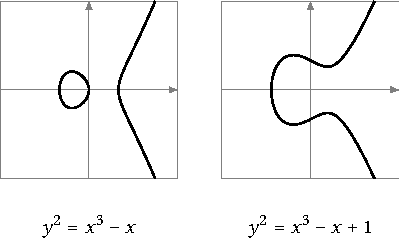
\includegraphics[width=.75\textwidth]{img/ejemplos-curvas}
    \caption{Ejemplos de curvas elípticas sobre $\mathbb{R}$. Basado en \parencite{eichlseder_elliptic_2016}.}
    \label{fig:curva}
  \end{figure}
\end{frame}

\begin{frame}{Suma de puntos (I)}
  % Hablar de:
  % - método algebraico (lo que vamos a contar se hace con ecuaciones)
  % - el método geométrico lo vemos sobre R
  % - las rectas verticales cortan a la curva al menos en el punto del infinito
  \begin{itemize}
    \item Podemos definir una operación suma sobre los puntos de la curva para obtener un grupo abeliano.
    \item El elemento neutro será el punto \(\mathcal{O}\).
    %\item Vamos a ver el método geométrico sobre \(\mathbb R\).
  \end{itemize}
\end{frame}

\begin{frame}{Elemento inverso}
  \begin{figure}[h]
    \centering
    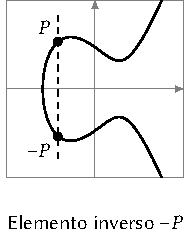
\includegraphics[width=0.35\textwidth]{img/inverso-curvas}
    \caption{Elemento inverso de un punto en curvas elípticas. Basado en  \parencite{eichlseder_elliptic_2016}.}
    \label{fig:inverso-curvas}
  \end{figure}  
\end{frame}

\begin{frame}{Suma de puntos}
  \begin{figure}[h]
    \centering
    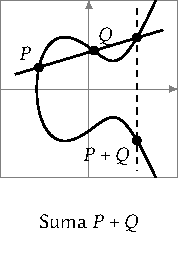
\includegraphics[width=0.35\textwidth]{img/suma-curvas}
    \caption{Suma de puntos en curvas elípticas. Basado en  \parencite{eichlseder_elliptic_2016}.}
    \label{fig:suma-curvas}
  \end{figure}  
\end{frame}

\begin{frame}{Duplicar puntos}
  \begin{figure}[h]
    \centering
    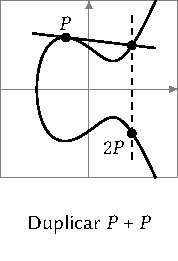
\includegraphics[width=0.35\textwidth]{img/duplicar-curvas}
    \caption{Duplicación de un punto en curvas elípticas. Basado en  \parencite{eichlseder_elliptic_2016}.}
    \label{fig:duplicar-curvas}
  \end{figure}  
\end{frame}

% TODO: Insertar figuras operaciones
% Decir que en cuerpos finitos que son los que se usan en criptografía se pone mod y aunque todo funcione igual es un poco más feo de ver

\begin{frame}[fragile]{Evolución de las curvas elípticas en la criptografía}{Años 70}
  \begin{itemize}
  \item En 1973 la NBS organizó un concurso público para el diseño de un algoritmo de cifrado que el Gobierno pudiera adoptar como estándar.
  \item En 1975 un grupo de investigación de IBM publicó el primer borrador del DES.
  \item La NSA aporta modificaciones y en 1976 la NBS lo aprobó y publicó. %contar que esto generó sospechas etc
  \item Este algoritmo fue reemplazado por AES en 2002.
  \end{itemize}
\end{frame}

\begin{frame}[fragile]{Evolución de las curvas elípticas en la criptografía}{Años 70}
  \begin{itemize}
  \item En 1976 se publicó el artículo \textit{New Directions in Cryptography} donde Diffie y Hellman proponen por primera vez la idea de cifrado de clave pública. % Explicar en una frase cifrado de clave pública y comentar que hasta el momento la seguridad de los algoritmos dependía solo de que solo los interesados conocieran la clave
   \item Explicar Diffie-Hellman...según vayamos de tiempo...si tenemos tiempo estaría bien porque simplificaría la explicación posterior del de curvas elípticas
  \end{itemize}
\end{frame}

\begin{frame}[fragile]{Evolución de las curvas elípticas en la criptografía}{Años 80}
\begin{itemize}
\item En 1984 H. Lenstra propone el primer algoritmo que utiliza las curvas elípticas, era un algoritmo de factorización.
\item En 1985 N. Koblitz y V. Miller proponen un criptosistema que usaba curvas elípticas basado en el problema del logaritmo discreto:
\begin{quote}
  Sea $E(\mathbb{F}_p)$ verificando $y^2 =x^3 + Ax + B$. Consideramos $\langle G \rangle$ un subgrupo cíclico de orden $n$ de los puntos de $E$. Dados $P,Q \in \langle G \rangle$ encuentra $x \bmod{n}$ tal que $Q=xP$.
  \end{quote}
\item Algoritmo ECDH. 
\end{itemize}
\end{frame}

\begin{frame}[fragile]{Evolución de las curvas elípticas en la criptografía}{Años 80}
\begin{itemize}
\item Se comienza a considerar este tipo de criptografía porque no se puede adaptar el \textit{index calculus} para calcular el logaritmo discreto en el grupo de una curva elíptica.
\item ¿Comentar lo de las curvas supersingulares?
\item Se adaptan los algoritmos existentes a este grupo.
\item En 1987 Koblitz adapta el algoritmo ElGamal.
\item ECDSA ¿año?, adaptación de DSA, algoritmo de firma.
\end{itemize}
\end{frame}

\begin{frame}[fragile]{Evolución de las curvas elípticas en la criptografía}{Años 80}
\begin{itemize}
\item Se desarrollan también algoritmos para resolver el problema del logaritmo discreto. % Aclarar que si se consiguiera el cifrado que lo usa no serviría
  % Los primeros adaptaban los algoritmos que existían en cuerpos finitos al grupo de la curva elíptica
\item Algoritmo de Pohlig y Hellman.
\item Algoritmo \textit{Baby-step/giant-step} de Shanks, \textit{rho} de Pollard. % Tiempo raíz de n
\item Ataque por emparejamiento de Weil. % SI se dice lo de las curvas supersingulares decir que este algoritmo es especialmente efectivo en ellas
\end{itemize}

% Durante los años siguientes a la aparición de la criptografía de la curva elíptica la actitud general de los criptógrafos fue de aceptación y curiosidad, nadie la consideró una amenaza comercial.
% A finales de los años 80, un grupo amplio de matemáticos empezó a trabajar en el tema ...
\end{frame}

\begin{frame}[fragile]{Evolución de las curvas elípticas en la criptografía}{Años 90 - Enfrentamiento con RSA - Apoyo de la NSA}
\begin{itemize}
\item RSA es un sistema de clave pública que apareció en 1977 y cuya seguridad radica en el problema de factorización. En este periodo ya comenzaba a tener éxito comercial. % estaba teniendo buena aceptación
\item Los partidarios de la ECC comienzan a luchar por la inclusión de los protocolos basados en curvas elípticas en los estándares criptográficos. (ECDSA no fue incluido hasta 1999 y 2000).
\item A principios de los 90 el NIST propuso un protocolo de firma desarrollado por la NSA donde la seguridad se basaba en el problema del logaritmo discreto.% Aunque este algoritmo, que se comercializó en 1994, no estaba basado en curvas elípticas, mostró el descontento con RSA que existía por parte de la NSA.
\item En 1997 RSA Data Security puso una sección en su página web advirtiendo del riesgo que suponía usar la criptografía basada en curvas elípticas. % Defensa de ECC , pero tenía el problema de que necesitaban claves cada vez más largas (algoritmo criba general del cuerpo de números)
  % ¿poner citas?
\item El mismo año  un miembro de la NSA publica
el primer artículo en un congreso sobre criptografía que trataba sobre la ECC.
\item Nuevo ataque para el problema del logaritmo discreto \textit{xedni} (1998). % ¿Esto tiene relevancia? No tengo claro si dice algo más allá de que es un algoritmo que serviría para romper los dos...
\end{itemize}
\end{frame}

\begin{frame}[fragile]{Evolución de las curvas elípticas en la criptografía}{Años 90 - Enfrentamiento con RSA - Apoyo de la NSA}
\begin{table}[h]
  \centering
  \sffamily
  \begin{tabular}{lccc}
    \toprule
     & \multicolumn{3}{c}{Tamaño en bits} \\
    Periodo & nivel de seguridad & RSA & ECC \\
    \midrule
    Pasado & 80 & 1024 & 160\\
    \multirow[t]{4}{*}{2016-2030} & 112 & 2048 & 224\\
     & 128 & 3072 & 256\\
     & 192 & 7680 & 384\\
     & 256 & 15360 & 512\\
    \bottomrule
  \end{tabular}
  \caption{Recomendaciones del NIST para el tamaño de las claves de RSA y ECC. Un nivel de seguridad de \(S\) bits indica que se necesitan aproximadamente \(2^S\) operaciones para romper el cifrado.}
  \label{tab:rsa-ecc-nist}
\end{table} %Arreglar
\end{frame}


\begin{frame}
  \printbibliography
\end{frame}

\end{document}

